\documentclass[10pt,a4paper]{article}
\usepackage[margin=18mm]{geometry}
\usepackage[T1]{fontenc}
\usepackage{lmodern,microtype}
\usepackage{amsmath,amssymb,booktabs,graphicx}
\usepackage[hidelinks]{hyperref}
\usepackage{caption}
\captionsetup{font=small,labelfont=bf}
\setlength{\parskip}{4pt}
\setlength{\parindent}{0pt}
\setlength{\emergencystretch}{2em}
% Generated by scripts/cellbridge_numbers_v100.py. Do not edit by hand.
\newcommand{\Num}[1]{#1}
\newcommand{\NGseTrain}{11}
\newcommand{\NGseCal}{9}
\newcommand{\NGseTest}{10}
\newcommand{\NEmTrain}{64}
\newcommand{\NEmCal}{31}
\newcommand{\NEmTest}{29}
\newcommand{\MaeGseCbEone}{0.284}
\newcommand{\MaeGseCbEtwo}{0.322}
\newcommand{\MaeGseAbEone}{0.315}
\newcommand{\MaeGseAbEtwo}{0.359}
\newcommand{\MaeGseTvEone}{0.393}
\newcommand{\MaeGseTvEtwo}{0.395}
\newcommand{\MaeGseRoEone}{0.376}
\newcommand{\MaeGseRoEtwo}{0.461}
\newcommand{\MaeGseJtEone}{0.756}
\newcommand{\MaeGseJtEtwo}{0.722}
\newcommand{\MaeGseRnEone}{0.799}
\newcommand{\MaeGseRnEtwo}{0.755}
\newcommand{\MaeGseMnEone}{0.511}
\newcommand{\MaeGseMnEtwo}{0.643}
\newcommand{\MaeEmCbEone}{0.530}
\newcommand{\MaeEmCbEtwo}{0.471}
\newcommand{\MaeEmAbEone}{0.526}
\newcommand{\MaeEmAbEtwo}{0.472}
\newcommand{\MaeEmTvEone}{0.929}
\newcommand{\MaeEmTvEtwo}{0.844}
\newcommand{\MaeEmRoEone}{0.889}
\newcommand{\MaeEmRoEtwo}{0.815}
\newcommand{\MaeEmJtEone}{0.889}
\newcommand{\MaeEmJtEtwo}{0.824}
\newcommand{\MaeEmRnEone}{0.889}
\newcommand{\MaeEmRnEtwo}{0.824}
\newcommand{\MaeEmMnEone}{0.889}
\newcommand{\MaeEmMnEtwo}{0.824}
\newcommand{\GseHOneGain}{0.321}
\newcommand{\GseHOneLo}{0.238}
\newcommand{\GseHOneHi}{0.410}
\newcommand{\GseHOneP}{=0.002}
\newcommand{\GseHOneWins}{10}
\newcommand{\GseHOneN}{10}
\newcommand{\GseHOneTested}{tested}
\newcommand{\GseHOneCall}{rejected}
\newcommand{\GseHTwoGain}{0.400}
\newcommand{\GseHTwoLo}{0.158}
\newcommand{\GseHTwoHi}{0.682}
\newcommand{\GseHTwoP}{=0.006}
\newcommand{\GseHTwoWins}{9}
\newcommand{\GseHTwoN}{10}
\newcommand{\GseHTwoTested}{tested}
\newcommand{\GseHTwoCall}{rejected}
\newcommand{\GseHThreeGain}{0.432}
\newcommand{\GseHThreeLo}{0.169}
\newcommand{\GseHThreeHi}{0.742}
\newcommand{\GseHThreeP}{=0.006}
\newcommand{\GseHThreeWins}{9}
\newcommand{\GseHThreeN}{10}
\newcommand{\GseHThreeTested}{tested}
\newcommand{\GseHThreeCall}{rejected}
\newcommand{\GseHFourGain}{0.227}
\newcommand{\GseHFourLo}{0.142}
\newcommand{\GseHFourHi}{0.305}
\newcommand{\GseHFourP}{=0.004}
\newcommand{\GseHFourWins}{9}
\newcommand{\GseHFourN}{10}
\newcommand{\GseHFourTested}{tested}
\newcommand{\GseHFourCall}{rejected}
\newcommand{\GseHFiveGain}{0.472}
\newcommand{\GseHFiveLo}{0.198}
\newcommand{\GseHFiveHi}{0.771}
\newcommand{\GseHFiveP}{=0.002}
\newcommand{\GseHFiveWins}{10}
\newcommand{\GseHFiveN}{10}
\newcommand{\GseHFiveTested}{tested}
\newcommand{\GseHFiveCall}{rejected}
\newcommand{\GseHSixGain}{0.516}
\newcommand{\GseHSixLo}{0.218}
\newcommand{\GseHSixHi}{0.846}
\newcommand{\GseHSixP}{=0.002}
\newcommand{\GseHSixWins}{10}
\newcommand{\GseHSixN}{10}
\newcommand{\GseHSixTested}{tested}
\newcommand{\GseHSixCall}{rejected}
\newcommand{\GseHSevenGain}{0.072}
\newcommand{\GseHSevenLo}{0.032}
\newcommand{\GseHSevenHi}{0.113}
\newcommand{\GseHSevenP}{=0.010}
\newcommand{\GseHSevenWins}{9}
\newcommand{\GseHSevenN}{10}
\newcommand{\GseHSevenTested}{tested}
\newcommand{\GseHSevenCall}{rejected}
\newcommand{\GseHEightGain}{0.109}
\newcommand{\GseHEightLo}{0.043}
\newcommand{\GseHEightHi}{0.183}
\newcommand{\GseHEightP}{=0.016}
\newcommand{\GseHEightWins}{8}
\newcommand{\GseHEightN}{10}
\newcommand{\GseHEightTested}{tested}
\newcommand{\GseHEightCall}{rejected}
\newcommand{\GseHNineGain}{0.037}
\newcommand{\GseHNineLo}{-0.003}
\newcommand{\GseHNineHi}{0.085}
\newcommand{\GseHNineP}{=0.154}
\newcommand{\GseHNineWins}{7}
\newcommand{\GseHNineN}{10}
\newcommand{\GseHNineTested}{tested}
\newcommand{\GseHNineCall}{not rejected}
\newcommand{\GseHTenGain}{0.032}
\newcommand{\GseHTenLo}{-0.050}
\newcommand{\GseHTenHi}{0.113}
\newcommand{\GseHTenP}{=0.492}
\newcommand{\GseHTenWins}{5}
\newcommand{\GseHTenN}{10}
\newcommand{\GseHTenTested}{not tested in sequence}
\newcommand{\GseHTenCall}{not rejected}
\newcommand{\GseNiEoneUpper}{0.050}
\newcommand{\GseNiEoneHold}{held}
\newcommand{\GseNiEtwoUpper}{0.003}
\newcommand{\GseNiEtwoHold}{held}
\newcommand{\GseCovCb}{0.883}
\newcommand{\EmHOneGain}{0.353}
\newcommand{\EmHOneLo}{0.108}
\newcommand{\EmHOneHi}{0.668}
\newcommand{\EmHOneP}{<0.001}
\newcommand{\EmHOneWins}{21}
\newcommand{\EmHOneN}{29}
\newcommand{\EmHOneTested}{tested}
\newcommand{\EmHOneCall}{rejected}
\newcommand{\EmHTwoGain}{0.353}
\newcommand{\EmHTwoLo}{0.108}
\newcommand{\EmHTwoHi}{0.668}
\newcommand{\EmHTwoP}{<0.001}
\newcommand{\EmHTwoWins}{21}
\newcommand{\EmHTwoN}{29}
\newcommand{\EmHTwoTested}{tested}
\newcommand{\EmHTwoCall}{rejected}
\newcommand{\EmHThreeGain}{0.353}
\newcommand{\EmHThreeLo}{0.108}
\newcommand{\EmHThreeHi}{0.668}
\newcommand{\EmHThreeP}{<0.001}
\newcommand{\EmHThreeWins}{21}
\newcommand{\EmHThreeN}{29}
\newcommand{\EmHThreeTested}{tested}
\newcommand{\EmHThreeCall}{rejected}
\newcommand{\EmHFourGain}{0.359}
\newcommand{\EmHFourLo}{0.032}
\newcommand{\EmHFourHi}{0.780}
\newcommand{\EmHFourP}{=0.061}
\newcommand{\EmHFourWins}{16}
\newcommand{\EmHFourN}{29}
\newcommand{\EmHFourTested}{tested}
\newcommand{\EmHFourCall}{not rejected}
\newcommand{\EmHFiveGain}{0.359}
\newcommand{\EmHFiveLo}{0.032}
\newcommand{\EmHFiveHi}{0.780}
\newcommand{\EmHFiveP}{=0.061}
\newcommand{\EmHFiveWins}{16}
\newcommand{\EmHFiveN}{29}
\newcommand{\EmHFiveTested}{not tested in sequence}
\newcommand{\EmHFiveCall}{not rejected}
\newcommand{\EmHSixGain}{0.359}
\newcommand{\EmHSixLo}{0.032}
\newcommand{\EmHSixHi}{0.780}
\newcommand{\EmHSixP}{=0.061}
\newcommand{\EmHSixWins}{16}
\newcommand{\EmHSixN}{29}
\newcommand{\EmHSixTested}{not tested in sequence}
\newcommand{\EmHSixCall}{not rejected}
\newcommand{\EmHSevenGain}{0.374}
\newcommand{\EmHSevenLo}{0.113}
\newcommand{\EmHSevenHi}{0.707}
\newcommand{\EmHSevenP}{<0.001}
\newcommand{\EmHSevenWins}{21}
\newcommand{\EmHSevenN}{29}
\newcommand{\EmHSevenTested}{not tested in sequence}
\newcommand{\EmHSevenCall}{not rejected}
\newcommand{\EmHEightGain}{0.399}
\newcommand{\EmHEightLo}{0.062}
\newcommand{\EmHEightHi}{0.824}
\newcommand{\EmHEightP}{=0.030}
\newcommand{\EmHEightWins}{18}
\newcommand{\EmHEightN}{29}
\newcommand{\EmHEightTested}{not tested in sequence}
\newcommand{\EmHEightCall}{not rejected}
\newcommand{\EmHNineGain}{0.001}
\newcommand{\EmHNineLo}{-0.028}
\newcommand{\EmHNineHi}{0.029}
\newcommand{\EmHNineP}{=0.931}
\newcommand{\EmHNineWins}{15}
\newcommand{\EmHNineN}{29}
\newcommand{\EmHNineTested}{not tested in sequence}
\newcommand{\EmHNineCall}{not rejected}
\newcommand{\EmHTenGain}{-0.003}
\newcommand{\EmHTenLo}{-0.073}
\newcommand{\EmHTenHi}{0.065}
\newcommand{\EmHTenP}{=0.931}
\newcommand{\EmHTenWins}{14}
\newcommand{\EmHTenN}{29}
\newcommand{\EmHTenTested}{not tested in sequence}
\newcommand{\EmHTenCall}{not rejected}
\newcommand{\EmNiEoneUpper}{0.073}
\newcommand{\EmNiEoneHold}{did not hold}
\newcommand{\EmNiEtwoUpper}{0.028}
\newcommand{\EmNiEtwoHold}{held}
\newcommand{\EmCovCb}{0.926}
\newcommand{\EmStopped}{H4}
\newcommand{\GseClaim}{supported}
\newcommand{\EmClaim}{not supported}
\newcommand{\MetaMnFe}{0.324}
\newcommand{\MetaMnSe}{0.044}
\newcommand{\MetaMnRe}{0.324}
\newcommand{\MetaMnReSe}{0.044}
\newcommand{\MetaJtFe}{0.377}
\newcommand{\MetaJtSe}{0.102}
\newcommand{\MetaJtRe}{0.377}
\newcommand{\MetaJtReSe}{0.102}
\newcommand{\MetaRnFe}{0.391}
\newcommand{\MetaRnSe}{0.106}
\newcommand{\MetaRnRe}{0.391}
\newcommand{\MetaRnReSe}{0.106}
\newcommand{\MetaTvFe}{0.078}
\newcommand{\MetaTvSe}{0.021}
\newcommand{\MetaTvRe}{0.183}
\newcommand{\MetaTvReSe}{0.145}
\newcommand{\MetaAbFe}{0.012}
\newcommand{\MetaAbSe}{0.013}
\newcommand{\MetaAbRe}{0.015}
\newcommand{\MetaAbReSe}{0.017}
\newcommand{\DevCb}{0.777}
\newcommand{\DevAb}{0.896}
\newcommand{\DevJt}{0.985}
\newcommand{\DevRn}{0.988}
\newcommand{\DevMn}{1.032}
\newcommand{\AblFull}{0.777}
\newcommand{\AblAnchor}{0.774}
\newcommand{\AblKone}{0.781}
\newcommand{\AblRho}{0.782}
\newcommand{\AblRna}{0.862}
\newcommand{\PanelZero}{0.859}
\newcommand{\PanelOne}{0.800}
\newcommand{\PanelTwo}{0.780}
\newcommand{\PanelFour}{0.760}
\newcommand{\PanelEight}{0.766}
\newcommand{\SimCells}{0.18}
\newcommand{\SimKmeans}{0.19}
\newcommand{\SimOracle}{0.76}
\newcommand{\SimCov}{0.895}
\newcommand{\BootCdOneFiveFour}{85}
\newcommand{\BootCdTwentyFive}{85}
\newcommand{\BootCdSixtyNine}{80}
\newcommand{\GseTvCells}{89,906}
\newcommand{\GseTvQuery}{149,666}
\newcommand{\EmTvCells}{144,723}
\newcommand{\EmTvGenes}{4,023}
\newcommand{\EmLr}{$4\times 10^{-4}$}
\newcommand{\GseCbSeconds}{9.2}
\newcommand{\GseTvSeconds}{2350}
\newcommand{\GseTvMinutes}{39}
\newcommand{\EmTvSeconds}{3983}
\newcommand{\EmTvMinutes}{66}
\newcommand{\ScaleMillionSeconds}{3.1}

\title{\bfseries CellBridge: supplementary methods and figures}
\author{Arman Salehi}
\date{}
\begin{document}
\maketitle

\section{Profiled estimator}
Start from the cell model in the main text. Stack the cells of one target and write the design as donor indicators, an arm indicator and the features \(Z\). The donor intercepts and the arm intercept are unpenalised. For a fixed slope \(\beta\), their least-squares estimates are the arm-wise means of the residual \(y-Z\beta\). Substituting those estimates back into an arm-balanced squared loss removes them. What remains is a within-arm scatter of the cells, or of the metacell means, plus a between-arm term that depends on the donor-level responses only.

The weight \(\rho\) multiplies the between-arm term. The ridge penalty is applied after the features and the within-arm response have been standardised, so \(\lambda\) is comparable across proteins. The standardised within-arm matrix is factorised once for each feature set and metacell size. Every pair \((\rho,\lambda)\) is then a rank-\(D\) Woodbury update, where \(D\) is the number of training donors. Mapping the standardised slope back to the original features gives \(\beta\). Equation~(2) of the main text is the mean of that linear predictor over the cells of a query donor, which collapses to the donor's mean feature change. No further approximation is required. Averaging the slopes of the selected configurations keeps the same identity, so the feature contributions still sum to the prediction.

As \(\lambda\) grows, \(\beta\) shrinks to zero and the prediction tends to the training-donor mean response \(m_y\). That is why a ridge that selects a very large penalty can match the training mean exactly, as both pseudobulk ridges did on E-MTAB-9357.

\section{Abundance-shrinkage baseline}
The baseline that the main text calls abundance shrinkage is not refit as part of CellBridge. It learns a linear map from RNA to protein using the abundance in each condition, then uses the eight anchor responses to shrink the residual of the paired response. Its penalty and shrinkage are chosen on the training donors only, on the same inner split as the other baselines. On a query donor it sees RNA and the anchor responses, not the hidden proteins. Full implementation details are in the frozen source \texttt{abundance\_response.py} and \texttt{shrinkage.py}, which the GSE334503 freeze hashes.

\section{Protocols and chronology}
GSE334503 was frozen, fit, sealed and unblinded once under \texttt{configs/protocol\_cellbridge\_v100.json}. The seal time recorded on the laptop is 2026-10-07T12:46:56.735401+00:00. That timestamp is the laptop clock until the archive is deposited.

E-MTAB-9357 uses \texttt{configs/protocol\_cellbridge\_v100\_emtab9357.json} and \texttt{docs/prereg\_emtab9357.md}. The freeze checks the solver hashes against the GSE334503 freeze before any E-MTAB outcome is opened. Panel aliases, such as CD279 to PD-1 and CD278 to ICOS, live only in the cohort adapter. The OSF URL was null when the protocol was hashed.

v0.5 of the surrounding project was superseded, and the all-protein endpoint E2 was added, before the GSE334503 unblind. Those earlier predictions were not used to choose the v1.0 grid. E-MTAB-9357 patient roles were locked from metadata. Eligibility uses RNA-labelled T cells only. The replication rejected H1--H3 and stopped at H4. Non-inferiority to abundance shrinkage \EmNiEtwoHold{} on E2 and \EmNiEoneHold{} on E1.

\section{totalVI settings}
Both fits use scvi-tools TOTALVI, latent distribution normal, batch key equal to the donor, 200 maximum epochs, batch size 256, at most 1{,}500 cells per donor-arm and 10 posterior samples at prediction. Query proteins other than the anchors are zeros. \texttt{transform\_batch} is the list of training donors. Early stopping uses the package default.

GSE334503 was fit on raw counts. The fit took \GseTvSeconds{} seconds on \GseTvCells{} cells. E-MTAB-9357 matrices are \(\log(1+\mathrm{CPM})\). Counts were \(\mathrm{round}(\mathrm{expm1}(x)/100)\). The learning rate was \EmLr{} rather than the package default \(4\times 10^{-3}\). Both choices were fixed because the encoder produced non-finite values during training, and both were fixed before the outcome vault was opened. The fit then completed 200 epochs in \EmTvSeconds{} seconds. Training curves are in Figure~\ref{fig:s3}. The early spike in the E-MTAB validation curve recovered; the run was not restarted.

\section{Ablations, simulation and scaling}
The nine-task means in the main text are computed from \texttt{analysis/development/summary.csv} and from the reduced-grid file \texttt{open\_ablations/subgrid\_means.csv}. The panel curve and the gene curve use the same exploratory grid and were not used to change the locked anchors or the locked gene count. Figure~\ref{fig:s4} shows the gene curve. From about 100 genes to about 2{,}000, the nine-task mean moves only between the values stored in that file.

Figure~\ref{fig:s2} is a simulation with a known slope and noisy features. At noise scale 2, averaging cells that share the latent state recovers a slope norm ratio of \SimOracle{}. Single cells recover \SimCells{}, and \(k\)-means on the noisy features recovers \SimKmeans{}. Metacells help when the grouping tracks cell state. They do not help when the grouping is only a clustering of the noisy features. The inner loop is free to put weight on \(k=1\). In the same simulation, split-conformal intervals covered \SimCov{} of 200 exchangeable draws at a nominal coverage of 0.9.

Per-protein errors on the two sealed tests are in Figure~\ref{fig:s1}. They are descriptive. They were computed from the sealed predictions and the outcomes the single unblind had already opened, and they were not used to change a hypothesis.

\begin{figure}[t]
\centering
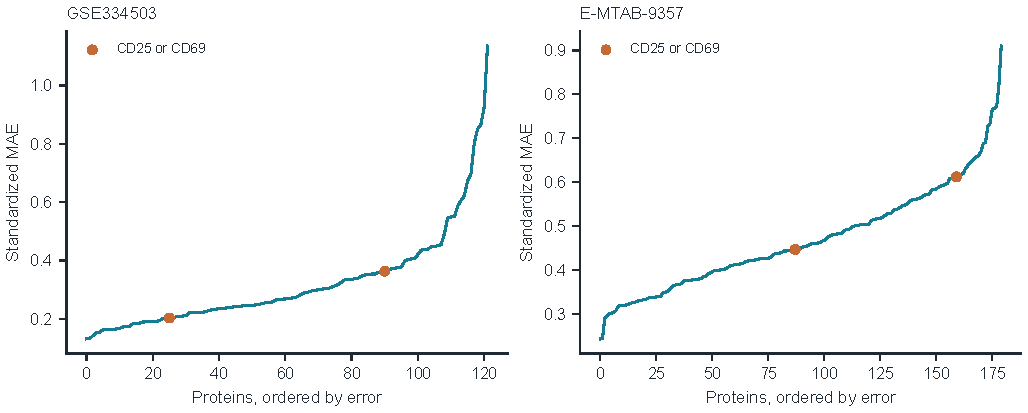
\includegraphics[width=\textwidth]{figures/figureS1_per_protein.pdf}
\caption{CellBridge standardized MAE by protein, ordered within each cohort. Orange points are CD25 and CD69.}
\label{fig:s1}
\end{figure}

\begin{figure}[t]
\centering
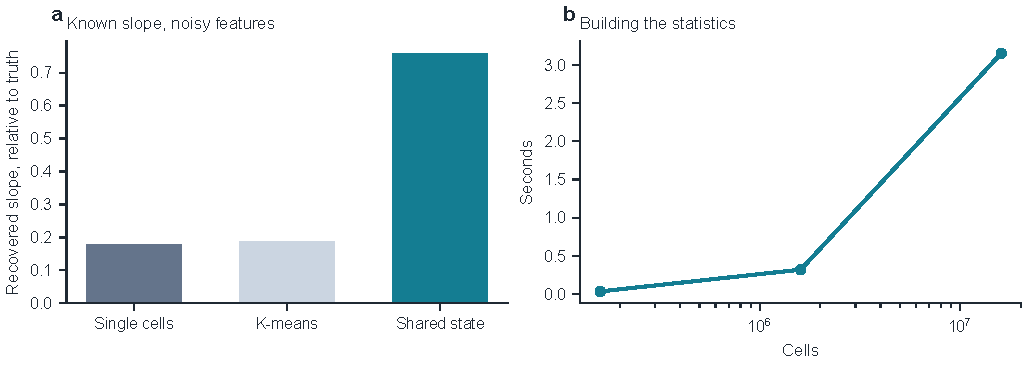
\includegraphics[width=\textwidth]{figures/figureS2_simulation.pdf}
\caption{\textbf{(a)} Recovery of a known slope at noise scale 2. \textbf{(b)} Time to build and fit the sufficient statistics as the number of cells grows. Eight donors, 30 features.}
\label{fig:s2}
\end{figure}

\begin{figure}[t]
\centering
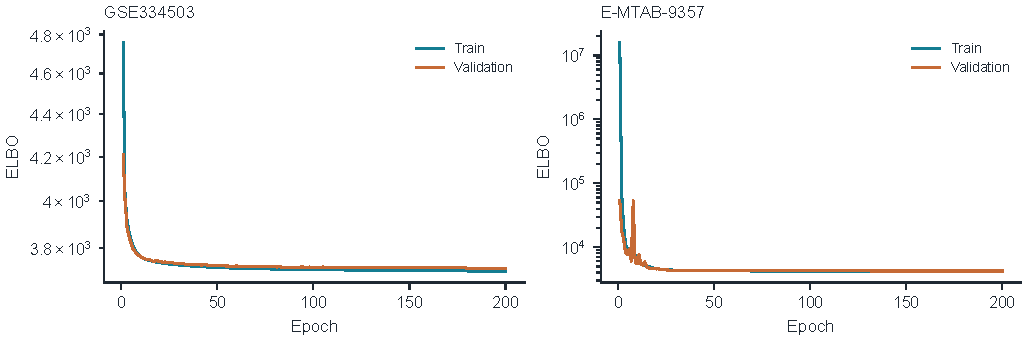
\includegraphics[width=\textwidth]{figures/figureS3_totalvi.pdf}
\caption{totalVI evidence lower bound on the two sealed fits. The vertical scale is logarithmic.}
\label{fig:s3}
\end{figure}

\begin{figure}[t]
\centering
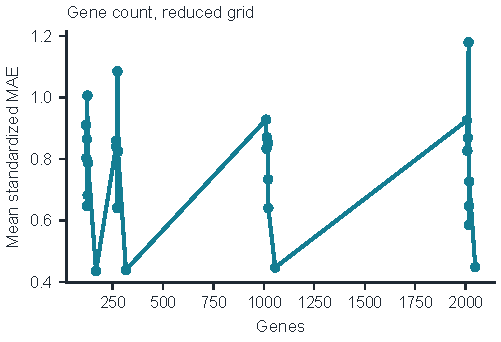
\includegraphics[width=0.72\textwidth]{figures/figureS4_genes.pdf}
\caption{Gene count on the reduced exploratory grid. Each point is the mean over the nine development tasks.}
\label{fig:s4}
\end{figure}

\section{Meta-analysis, fixed effect}
For all hidden proteins, the inverse-variance fixed effects were \MetaMnFe{} (SE \MetaMnSe{}) against the mean, \MetaJtFe{} (SE \MetaJtSe{}) against the joint ridge, \MetaRnFe{} (SE \MetaRnSe{}) against the RNA ridge, \MetaTvFe{} (SE \MetaTvSe{}) against totalVI and \MetaAbFe{} (SE \MetaAbSe{}) against abundance shrinkage. Random effects are in the main text. The analysis does not change the fixed sequence of either cohort.

\section{Limits restated}
Lawlor was previously exposed. The sealed cohorts are small. Attributions are predictive, not causal. E-MTAB-9357 inputs for the comparators are reconstructed CPM, not raw UMIs. totalVI on that cohort used the scaled counts and learning rate above. The GSE334503 seal time is local until the archive is uploaded. The E-MTAB-9357 OSF URL was null at the freeze.
\end{document}
